% Template for PLoS
% Version 3.3 June 2016
%
% % % % % % % % % % % % % % % % % % % % % %
%
% -- IMPORTANT NOTE
%
% This template contains comments intended 
% to minimize problems and delays during our production 
% process. Please follow the template instructions
% whenever possible.
%
% % % % % % % % % % % % % % % % % % % % % % % 
%
% Once your paper is accepted for publication, 
% PLEASE REMOVE ALL TRACKED CHANGES in this file 
% and leave only the final text of your manuscript. 
% PLOS recommends the use of latexdiff to track changes during review, as this will help to maintain a clean tex file.
% Visit https://www.ctan.org/pkg/latexdiff?lang=en for info or contact us at latex@plos.org.
%
%
% There are no restrictions on package use within the LaTeX files except that 
% no packages listed in the template may be deleted.
%
% Please do not include colors or graphics in the text.
%
% The manuscript LaTeX source should be contained within a single file (do not use \input, \externaldocument, or similar commands).
%
% % % % % % % % % % % % % % % % % % % % % % %
%
% -- FIGURES AND TABLES
%
% Please include tables/figure captions directly after the paragraph where they are first cited in the text.
%
% DO NOT INCLUDE GRAPHICS IN YOUR MANUSCRIPT
% - Figures should be uploaded separately from your manuscript file. 
% - Figures generated using LaTeX should be extracted and removed from the PDF before submission. 
% - Figures containing multiple panels/subfigures must be combined into one image file before submission.
% For figure citations, please use "Fig" instead of "Figure".
% See http://journals.plos.org/plosone/s/figures for PLOS figure guidelines.
%
% Tables should be cell-based and may not contain:
% - spacing/line breaks within cells to alter layout or alignment
% - do not nest tabular environments (no tabular environments within tabular environments)
% - no graphics or colored text (cell background color/shading OK)
% See http://journals.plos.org/plosone/s/tables for table guidelines.
%
% For tables that exceed the width of the text column, use the adjustwidth environment as illustrated in the example table in text below.
%
% % % % % % % % % % % % % % % % % % % % % % % %
%
% -- EQUATIONS, MATH SYMBOLS, SUBSCRIPTS, AND SUPERSCRIPTS
%
% IMPORTANT
% Below are a few tips to help format your equations and other special characters according to our specifications. For more tips to help reduce the possibility of formatting errors during conversion, please see our LaTeX guidelines at http://journals.plos.org/plosone/s/latex
%
% For inline equations, please be sure to include all portions of an equation in the math environment.  For example, x$^2$ is incorrect; this should be formatted as $x^2$ (or $\mathrm{x}^2$ if the romanized font is desired).
%
% Do not include text that is not math in the math environment. For example, CO2 should be written as CO\textsubscript{2} instead of CO$_2$.
%
% Please add line breaks to long display equations when possible in order to fit size of the column. 
%
% For inline equations, please do not include punctuation (commas, etc) within the math environment unless this is part of the equation.
%
% When adding superscript or subscripts outside of brackets/braces, please group using {}.  For example, change "[U(D,E,\gamma)]^2" to "{[U(D,E,\gamma)]}^2". 
%
% Do not use \cal for caligraphic font.  Instead, use \mathcal{}
%
% % % % % % % % % % % % % % % % % % % % % % % % 
%
% Please contact latex@plos.org with any questions.
%
% % % % % % % % % % % % % % % % % % % % % % % %

\documentclass[10pt,letterpaper]{article}\usepackage[]{graphicx}\usepackage[]{color}
%% maxwidth is the original width if it is less than linewidth
%% otherwise use linewidth (to make sure the graphics do not exceed the margin)
\makeatletter
\def\maxwidth{ %
  \ifdim\Gin@nat@width>\linewidth
    \linewidth
  \else
    \Gin@nat@width
  \fi
}
\makeatother

\definecolor{fgcolor}{rgb}{0.345, 0.345, 0.345}
\newcommand{\hlnum}[1]{\textcolor[rgb]{0.686,0.059,0.569}{#1}}%
\newcommand{\hlstr}[1]{\textcolor[rgb]{0.192,0.494,0.8}{#1}}%
\newcommand{\hlcom}[1]{\textcolor[rgb]{0.678,0.584,0.686}{\textit{#1}}}%
\newcommand{\hlopt}[1]{\textcolor[rgb]{0,0,0}{#1}}%
\newcommand{\hlstd}[1]{\textcolor[rgb]{0.345,0.345,0.345}{#1}}%
\newcommand{\hlkwa}[1]{\textcolor[rgb]{0.161,0.373,0.58}{\textbf{#1}}}%
\newcommand{\hlkwb}[1]{\textcolor[rgb]{0.69,0.353,0.396}{#1}}%
\newcommand{\hlkwc}[1]{\textcolor[rgb]{0.333,0.667,0.333}{#1}}%
\newcommand{\hlkwd}[1]{\textcolor[rgb]{0.737,0.353,0.396}{\textbf{#1}}}%
\let\hlipl\hlkwb

\usepackage{framed}
\makeatletter
\newenvironment{kframe}{%
 \def\at@end@of@kframe{}%
 \ifinner\ifhmode%
  \def\at@end@of@kframe{\end{minipage}}%
  \begin{minipage}{\columnwidth}%
 \fi\fi%
 \def\FrameCommand##1{\hskip\@totalleftmargin \hskip-\fboxsep
 \colorbox{shadecolor}{##1}\hskip-\fboxsep
     % There is no \\@totalrightmargin, so:
     \hskip-\linewidth \hskip-\@totalleftmargin \hskip\columnwidth}%
 \MakeFramed {\advance\hsize-\width
   \@totalleftmargin\z@ \linewidth\hsize
   \@setminipage}}%
 {\par\unskip\endMakeFramed%
 \at@end@of@kframe}
\makeatother

\definecolor{shadecolor}{rgb}{.97, .97, .97}
\definecolor{messagecolor}{rgb}{0, 0, 0}
\definecolor{warningcolor}{rgb}{1, 0, 1}
\definecolor{errorcolor}{rgb}{1, 0, 0}
\newenvironment{knitrout}{}{} % an empty environment to be redefined in TeX

\usepackage{alltt}
\usepackage[top=0.85in,left=2.75in,footskip=0.75in]{geometry}

% amsmath and amssymb packages, useful for mathematical formulas and symbols
\usepackage{amsmath,amssymb}

% Use adjustwidth environment to exceed column width (see example table in text)
\usepackage{changepage}

% Use Unicode characters when possible
\usepackage[utf8x]{inputenc}

% textcomp package and marvosym package for additional characters
\usepackage{textcomp,marvosym}

% cite package, to clean up citations in the main text. Do not remove.
\usepackage{cite}

% Use nameref to cite supporting information files (see Supporting Information section for more info)
\usepackage{nameref,hyperref}

% line numbers
\usepackage[right]{lineno}

% ligatures disabled
\usepackage{microtype}
\DisableLigatures[f]{encoding = *, family = * }

% color can be used to apply background shading to table cells only
\usepackage[table]{xcolor}

% array package and thick rules for tables
\usepackage{array}

% create "+" rule type for thick vertical lines
\newcolumntype{+}{!{\vrule width 2pt}}

% create \thickcline for thick horizontal lines of variable length
\newlength\savedwidth
\newcommand\thickcline[1]{%
  \noalign{\global\savedwidth\arrayrulewidth\global\arrayrulewidth 2pt}%
  \cline{#1}%
  \noalign{\vskip\arrayrulewidth}%
  \noalign{\global\arrayrulewidth\savedwidth}%
}

% \thickhline command for thick horizontal lines that span the table
\newcommand\thickhline{\noalign{\global\savedwidth\arrayrulewidth\global\arrayrulewidth 2pt}%
\hline
\noalign{\global\arrayrulewidth\savedwidth}}


% Remove comment for double spacing
%\usepackage{setspace} 
%\doublespacing

% Text layout
\raggedright
\setlength{\parindent}{0.5cm}
\textwidth 5.25in 
\textheight 8.75in

% Bold the 'Figure #' in the caption and separate it from the title/caption with a period
% Captions will be left justified
\usepackage[aboveskip=1pt,labelfont=bf,labelsep=period,justification=raggedright,singlelinecheck=off]{caption}
\renewcommand{\figurename}{Fig}

% Use the PLoS provided BiBTeX style
\bibliographystyle{plos2015}

% Remove brackets from numbering in List of References
\makeatletter
\renewcommand{\@biblabel}[1]{\quad#1.}
\makeatother

% Leave date blank
\date{}

% Header and Footer with logo
\usepackage{lastpage,fancyhdr,graphicx}
\usepackage{epstopdf}
\pagestyle{myheadings}
\pagestyle{fancy}
\fancyhf{}
\setlength{\headheight}{27.023pt}
\lhead{
\includegraphics[width=2.0in]{PLOS-submission.eps}}
\rfoot{\thepage/\pageref{LastPage}}
\renewcommand{\footrule}{\hrule height 2pt \vspace{2mm}}
\fancyheadoffset[L]{2.25in}
\fancyfootoffset[L]{2.25in}
\lfoot{\sf PLOS}

%% Include all macros below

\newcommand{\lorem}{{\bf LOREM}}
\newcommand{\ipsum}{{\bf IPSUM}}

%% END MACROS SECTION

%% Added packages
\usepackage{adjustbox}
\usepackage{caption}
\usepackage{epstopdf}
\IfFileExists{upquote.sty}{\usepackage{upquote}}{}
\begin{document}
\vspace*{0.2in}

% Title must be 250 characters or less.
\begin{flushleft}
{\Large
\textbf\newline{A SuperLearner Ensemble Machine Learning Algorithm is Non-inferior to Clinicians in Prioritising Among Adult Trauma Patients in the Emergency Department: a Prospective Cohort Study in India} % Please use "title case" (capitalize all terms in the title except conjunctions, prepositions, and articles).
}
\newline
% Insert author names, affiliations and corresponding author email (do not include titles, positions, or degrees).
\\
Ludvig Wärnberg Gerdin\textsuperscript{1, \Yinyang},
Alan Hubbard\textsuperscript{2}, 
Anurag Mishra\textsuperscript{3}, 
Catherine Juillard\textsuperscript{4}, 
Debojit Basak\textsuperscript{5}, 
Deepa Kizhakke Veetil\textsuperscript{6}, 
Greeshma Abraham\textsuperscript{5}
Jyoti Kamble\textsuperscript{5},
Kapil Dev Soni\textsuperscript{7}, 
Makhan Lal Saha\textsuperscript{8}, 
Monty Khajanchi\textsuperscript{9}, 
Nitin Borle\textsuperscript{10},
Vineet Kumar\textsuperscript{11}, 
Sara Moore\textsuperscript{2}, 
Martin Gerdin Wärnberg\textsuperscript{12*\textcurrency, \Yinyang, \ddag}
\\
\bigskip
\textbf{1} KTH Royal Institute of Technology, Stockholm, Sweden
\\
\textbf{2} Division of Epidemiology and Biostatistics, School of Public Health, University of California, Berkeley, California, USA.
\\
\textbf{3} Department of Surgery, Maulana Azad Medical College, New Delhi, Delhi, India
\\
\textbf{4} Department of Surgery, Center for Global Surgical Studies, University of California, San Francisco, California, USA.
\\
\textbf{5} Tata Institute of Social Sciences and Doctors for You, Mumbai, Maharashtra, India
\\
\textbf{6} Department of General Surgery, Manipal hospital, Human Care Medical Charitable Trust, New Delhi, Delhi, India
\\
\textbf{7} Critical \& Intensive Care, JPN Apex Trauma Centre, All India Institute of Medical Sciences, New Delhi, Delhi, India
\\
\textbf{8} Department of Surgery, Institute of Post-Graduate Medical Education and Research and Seth Sukhlal Karnani Memorial Hospital, Kolkata, West Bengal, India
\\
\textbf{9} Department of Surgery, Seth Gowardhandas Sunderdas Medical College and King Edward Memorial Hospital, Mumbai, Maharashtra, India
\\
\textbf{10} Department of Surgery, Khershedji Behramji Bhabha hospital, Mumbai, Maharashtra, India
\\
\textbf{11} Department of Surgery, Lokmanya Tilak Municipal General Hospital, Mumbai, Maharashtra, India
\\
\textbf{12} Global Health: Health Systems and Policy, Department of Public Health Sciences, Karolinska Institutet, Stockholm, Sweden
\bigskip

% Insert additional author notes using the symbols described below. Insert symbol callouts after author names as necessary.
% 
% Remove or comment out the author notes below if they aren't used.
%
% Primary Equal Contribution Note
\Yinyang These authors contributed equally to this work.

% Additional Equal Contribution Note
% Also use this double-dagger symbol for special authorship notes, such as senior authorship.
\ddag Senior authorship.

% Current address notes
\textcurrency Current Address: Martin Gerdin Wärnberg, Department of Public
Health Sciences, Karolinska Institutet, 171 77 Stockholm, Sweden

% change symbol to "\textcurrency a" if more than one current address note
% \textcurrency b Insert second current address 
% \textcurrency c Insert third current address

% Deceased author note
% \dag Deceased

% Group/Consortium Author Note
% \textpilcrow Membership list can be found in the Acknowledgments section.

% Use the asterisk to denote corresponding authorship and provide email address in note below.
* martin.gerdin@ki.se

\end{flushleft}
% Please keep the abstract below 300 words
\section*{Abstract}
\subsection*{Background}
A key component of trauma care is the process of prioritizing patients to match
level of care with clinical acuity. In many emergency departments in low
resource setting hospitals trauma patients arrive with no or little
prenotification. In such settings patients are often prioritised by clinicians
based on patients' presentation. We aimed to compare the performance of an
ensemble machine learning methodology called SuperLearner to that of clinician
gestalt based on patients’ presentation.

\subsection*{Methods and findings}
Our hypothesis was that the performance of the SuperLearner would be
non-inferior to that of clinician gestalt in terms of classification. We used
data from an ongoing prospective cohort study in three public hospitals in urban
India. Adult patients presenting to the emergency departments of these hospitals
with history of trauma were approached for enrolment. The outcome was all cause
mortality within 30 days of arrival to a participating centre. For the purpose
of this study, clinicians were instructed to assign patients to one of four
levels corresponding to clinical acuity. The SuperLearner included five machine
learners and was developed in a training sample and then compared to clinicians
in a test sample. Performance was compared in terms of reclassification and area
under the receiver operating characteristics curve (AUROCC). We concluded that
the SuperLearner was non-inferior to clinicians if the lower bound of the 95\%
confidence intervals (CI) of the net reclassification in events was not less
than -0.05. From 28 July 2016 to 21 November 2017 we approached a total of
5667 patients for enrolment. Out of these,
4545 patients consented, had a priority
level assigned by a clinician, and had complete outcome data and were therefore
included in subsequent analysis. A total of 404 (9\%)
patients died within 30 days. We used a temporal split to divide the cohort into
a training and test sample. The training sample included
3408 patients and the test sample 1137
patients. The AUROCCs of the priority levels assigned by the SuperLearner and
clinicians were 0.9574 and 0.8727
respectively. The difference in AUROCC was
-0.0846 (95\% CI -0.1228 - -0.0451). The net reclassification in events was
0.0114 (95\% CI -0.0185 - 0.0299) and in non-events 0.3500 (95\% CI 0.2405 - 0.6895).

\subsection*{Conclusions}
In terms of classification and discrimination an ensemble machine learning
algorithm developed using the SuperLearner was non-inferior in prioritising
among adult trauma patients in the ED compared to clinician gestalt based on
patients’ presentation.

% Please keep the Author Summary between 150 and 200 words
% Use first person. PLOS ONE authors please skip this step. 
% Author Summary not valid for PLOS ONE submissions.   
\section*{Author Summary}
\subsection*{Why was this study done?}
Trauma kills almost five million people each year. A majority of these deaths
occur in low resource settings. New methods are needed to prioritise among
trauma patients in the emergency department and quickly identify patients in
need of immediate care. Machine learning could potentially help to do so, but so
far the use of machine learning in trauma research has been slow. We aimed to
compare the performance of an ensemble machine learning methodology called
SuperLearner to that of clinician gestalt based on patients’ presentation.

\subsection*{What did the researchers do and find?}
We analysed data from 4545 adult trauma
patients who presented to emergency departments at three public hospitals in
urban India. Out of these 404 (9\%) patients died from any
cause within 30 days of arrival to a participating hospital. We used the
SuperLearner to combine multiple machine learners to assign priority levels to
included trauma patients based on demographic and clinical patient
characteristics. We asked clinicians to also assign priority levels to the same
patients and compared the performance of the SuperLearner and clinicians. We
found that the SuperLearner was non-inferior to clinicians.

\subsection*{What do these findings mean?}
Using an ensemble machine learning algorithm to prioritise among trauma patients
in the ED may allow clinicians to focus on treating patients. This would free
valuable resources that are particularly scarce in the low resource settings
where most trauma deaths occur.

\linenumbers

% Use "Eq" instead of "Equation" for equation citations.
\section*{Introduction}
Trauma is a major threat to population health globally
\cite{Brohi2017,GBD2017}. Every year about 4.6 million people die because of
trauma - a number that exceeds the total number of yearly deaths from HIV/AIDS,
malaria and tuberculosis combined. The most common cause of trauma is road
traffic injuries (RTIs); in 2016 an estimated 1.3 million people died from RTIs
alone \cite{GBD2017}. Global actors have targeted a 50\% reduction of deaths
from road trauma by 2020, but this sustainable development goal is far from
being realized \cite{UN2018}. This situation calls for not only more
interventions, but also strengthened research on effective trauma care delivery.

Trauma care is highly time sensitive and delays to treatment have been
associated with increased mortality across settings
\cite{Yeboah2014,OReilly2013,Roy2017a}. Early identification and management of
potentially life threatening injuries are crucial for survival. A key component
of trauma care is therefore the process of prioritizing patients to match level
of care with clinical acuity \cite{EAST2010,NICE2016}. The existing literature
on how to prioritise trauma patients focuses largely on two issues. First, in
the prehospital setting the main focus has been to identify patients who merit
transfer to a trauma centre \cite{Voskens2018}. Second, in the hospital setting
a substantial body of research has focused on the appropriate criteria for
trauma team activation \cite{VanRein2018,Tignanelli2018}.

Although both these issues are important, clinicians all over the world are on a
daily basis faced with the more complex problem of how to decide in what order
to assess and treat trauma patients that arrive to the emergency department
(ED). In health systems with formalised criteria for prioritizing ED patients,
all patients are assigned a priority coupled with a target time to treat. These
priorities are may be coded with numbers \cite{ESI2012} or colors
\cite{SATG2012}, for example red, orange, yellow and green, with red being
assigned to the most urgent patients and green to the least urgent.

In health systems without formalized criteria, for example in many low resource
settings, clinician gestalt is used informally to prioritize among trauma
patients arriving to the ED \cite{Baker2013}. As there are commonly no formal
prehospital care systems in such settings, trauma patients often arrive to the
ED without warning and without any form of previous prioritisation to guide the
appropriate level of in-hospital care \cite{Choi2017}. Identifying ways to
quickly prioritize the patients in need of more immediate care would therefore
be very valuable in many low resource settings.

In contrast to trauma centre transfer or trauma team activation, the approach to
prioritization among trauma patients arriving to the ED has received little
attention from the research community. Framed as a classification problem this
challenge can be addressed using a statistical learner. Logistic or proportional
hazards models are common classification learners whereas more modern
alternatives include random forests or convolutional neural networks. These
learners all exist along the machine learning spectrum governed by their
relative ``human-to-machine decision-making-effort'', with regression learners
in the more-human-than-machine (MHTM) end and networks at the other, more
machine than human (MMTH), end of the spectrum \cite{Beam2018}.

MMTH learners have been used to solve classification problems in other fields of
medicine \cite{Nevin2018}, but the uptake and use of such learners in trauma
research has been slow \cite{Liu2017}. Some studies have approached the trauma
centre transfer and trauma team activation issues using MMTH learners, and the
results are conflicting with regards to the superiority of such learners over
MHTM learners or standard criteria
\cite{Talbert2007,Pearl2008,Scerbo2014,Follin2016}. One very recent study used a
random forest learner to assign priority to patients in a general ED population,
and found a slight performance improvement using this MMTH learner compared to
the standard criteria \cite{Levin2018}.

Given the paucity of research leveraging machine learning to prioritise among
trauma patients in the ED, we aimed to compare the performance of an ensemble
machine learning methodology called SuperLearner to that of clinician gestalt
based on patients’ presentation. Our hypothesis was that the performance of the
SuperLearner would be non-inferior to that of clinician gestalt.

% ** Materials and Methods
\section*{Materials and Methods}
% *** Study Design
\subsection*{Study Design}
We used data from an ongoing prospective cohort at three public hospitals in
urban India. Our analysis is an adjunct to a registered observational study to
compare the performance of clinical prediction models with clinicians
(ClinicalTrials.gov identifier NCT02838459).

% *** Setting
\subsection*{Study Setting}
Data analysed for this study came from patients enrolled between 28 July 2016
and 21 November 2017 at the three hospitals Khershedji Behramji Bhabha hospital
(KBBH) in Mumbai, Lok Nayak Hospital of Maulana Azad Medical College (MAMC) in
Delhi, and the Institute of Post-Graduate Medical Education and Research and
Seth Sukhlal Karnani Memorial Hospital (SSKM) in Kolkata. The time frame was
decided to ensure that all included patients had completed six months follow
up. KBBH is a community hospital with 436 inpatient beds. There are departments
of surgery, orthopaedics, anaesthesia, and both adult and paediatric intensive
care units. It has a general ED where all patients are seen. Most patients
present directly and are not transferred from another health centre. Plain
X-rays and ultrasonography are available around the clock but computed
tomography (CT) is only available in-house during day-time. During evenings and
nights patients in need of a CT are referred elsewhere. MAMC and SSKM are both
university and tertiary referral hospitals. This means that all specialities and
imaging facilities relevant to trauma care, except emergency medicine, are
available in-house around the clock. MAMC has approximately 2200 inpatient beds
and SSKM has around 1775 inpatient beds. Both MAMC and SSKM have general
EDs. Because both MAMC and SSKM are tertiary referral hospitals a large
proportion of patients arriving at their EDs are transferred from other health
facilities, with almost no transfer protocols in place. Prehospital care is
rudimentary in all three cities, with no organised emergency medical
services. Ambulances are predominately used for inter-hospital transfers and
most patients who arrive directly from the scene of the incident are brought by
the police or in private vehicles. Patients arriving to the ED are at all
centres first seen by a casualty medical officer on a largely first come first
served basis. There is no formalised system for prioritising ED patients at any
of the centres. The research was approved by the ethical review board at each
participating hospital. The names of the boards and the approval numbers were
Ethics and Scientific Committee (KBBH, HO/4982/KBB), the Institutional Ethics
Committee (MAMC, F.1/IEC/MAMC/53/2/2016/No97), and the IPGME\&R Research
Oversight Committee (SSKM, Inst/IEC/2016/328).

% *** Data Collection
\subsection*{Data Collection}
Data were collected by one dedicated project officer at each site. The project
officers all had a masters degree in life sciences. They worked five shifts per
week, and each shift was about eight hours long, so that mornings, evenings and
nights were covered according to a rotating schedule. In each shift, project
officers spent approximately six hours collecting data in the ED and the
remaining two following up patients. The collected data were then transferred
this data to a digital database. The rationale for this setup was to ensure
collection of high-quality data from a representative sample of trauma patients
arriving to the EDs at participating centres, while keeping to the projects
budget constraints.

% *** Participants
\subsection*{Participants}
\subsubsection*{Eligibility criteria}
Any person aged $\geq$ 18 years or older and who presented alive to the
emergency department (ED) of participating sites with history of trauma was
included. The age cutoff was chosen to align with Indian laws on research ethics
and informed consent. We defined history of trauma as having any of the external
causes of morbidity and mortality listed in block V01-Y36, chapter XX of the
International Classification of Disease version 10 (ICD-10) code book as primary
complaint. Drownings, inhalation and ingestion of objects causing obstruction of
respiratory tract, contact with venomous snakes and lizards, accidental
poisoning by and exposure to drugs, and overexertion were excluded because they
are not considered trauma at the participating centres.

\subsubsection*{Source and methods of selection of participants and follow up}
The project officers enrolled the first ten consecutive patients who presented
to the ED during each shift. The number of patients to enrol was set to ten to
make follow up feasible. Written informed consent from the patient or a patient
representative was obtained either in the ED or in the ward if the patient was
admitted. A follow-up was completed by the project officer 30 days and 6 months
after participant arrived at participating hospital. The follow-up was completed
in person or on phone, depending on whether the patient was still hospitalised
or if the patient had been discharged. Phone numbers of one or more contact
persons (e.g. relatives), were collected on enrolment and contacted if the
participant did not reply on follow up. Only if neither the participant nor the
contact person answered any of three repeated phone calls was the outcome
recorded as missing and the patient was considered lost to follow up.

% *** Variables, Data Sources and Measurement
\subsection*{Variables, Data Sources and Measurement}
\subsubsection*{Patient characteristics and SuperLearner variables}
The dependent variable, or label, used to train the SuperLearner was all-cause
30 day mortality, defined as death from any cause within 30 days of arrival to a
participating centre. These data were extracted from patient records if the
patient was still in hospital 30 days after arrival, or collected by calling the
patient or the patient representative if the patient was not in hospital.

The independent variables, or features, included patient age in years, sex,
mechanism of injury, type of injury, mode of transport, transfer status, time
from injury to arrival in hours. The project officers collected data on these
features by asking the patient, a patient representative, or by extracting the
data from the patient's file. Sex was coded as male or female. Mechanism of
injury was coded by the project officers using ICD-10 after completing the World
Health Organization's (WHO) electronic ICD-10-training tool \cite{WHOICD}. The
levels of mechanism of injury was collapsed for analysis into transport accident
(codes V00-V99), falls (W00-W19), burns (X00-X19), intentional self harm
(X60-X84), assault (X85-X99 and Y00-Y09), and other mechanism (W20-99, X20-59
and Y10-36). Type of injury was coded as blunt, penetrating, or both blunt and
penetrating. Mode of transport was coded as ambulance, police, private vehicle,
or arrived walking. Transfer status was a binary feature indicating if the
patient was transferred from another health facility or not.

The features also included vital signs measured on arrival to the ED at
participating centres. The project officers recorded all vital signs using hand
held equipment, i.e. these were not extracted from patient records, after
receiving two days of training and yearly refreshers. Only if the hand held
equipment failed to record a value did the project officers extract data from
other attached monitoring equipment, if available. Systolic and diastolic blood
pressure (SBP and DBP) were measured using an automatic blood pressure
monitor. Heart rate (HR) and peripheral capillary oxygen saturation
(SpO\textsubscript{2}) were measured using a portable non-invasive fingertip
pulse oximeter. Respiratory rate (RR) was measured manually by counting the
number of breaths during one minute. Level of consciousness was measured using
both the Glasgow coma scale (GCS) and the Alert, Voice, Pain, and Unresponsive
scale (AVPU). In assigning GCS the project officers used the official Glasgow
Coma Scale Assessment Aid \cite{GCSAID}. AVPU simply indicates whether the
patient is alert, responds to voice stimuli, painful stimuli, or does not
respond at all. These represent standard variables commonly collected in many
health systems. They are also included in several well known clinical prediction
models designed to predict trauma mortality \cite{Rehn2011}.

\subsubsection*{Clinicians' priority levels}
For the purpose of this study, clinicians were instructed by the project
officers to assign a priority to each patient. The priority levels were color
coded. Red was assigned to the most serious patients that should be treated
first. Green was assigned to the least serious patients that should be treated
last. Orange and yellow were intermediate levels, where orange patients were
less serious than red but more serious than yellow and green whereas yellow
patients were less serious than red and orange patients but more serious than
green patients. The clinicians were allowed to use all information available at
the time when they assigned the priority level, which was as soon as they had first
seen the patient. The priorities were not used to guide further patient care and
no interventions were implemented as part of the study for patients assigned to
the more urgent priority levels.

% *** Bias
\subsection*{Bias}
Project officers underwent two days of training in study procedures and were
then supervised locally. We conducted continuous data quality assurance by having
weekly online data review meetings during which data discrepancies were
identified, discussed and resolved. We conducted quarterly on site quality
control sessions during which data collection was conducted both by the centre's
own project officer and a quality control officer. Data entry errors were
prevented by having extensive logical checks in the digital data collection
instrument.

% *** Statistical methods
\subsection*{Statistical Methods}
All data was de-identified before it was analysed for this study. Details of the
de-identification procedures are available as supporting information in
\nameref{S1_Text}. We used R for all analyses \cite{R}. We first made a
non-random temporal split of the complete data set into a training and test
set. The split was made so that 75\% of the complete cohort was assigned to the
training set and the remaining 25\% to the test set, ensuring that the relative
contribution of each centre was maintained in both sets. We then calculated
descriptive statistics of all variables, using medians and inter quartile ranges
(IQR) for continuous variables and counts and percentages for qualitative
variables. All quantitative features (age, SBP, DBP, HR, SpO\textsubscript{2},
and RR) were treated as continuous and the levels of all qualitative variables
(sex, mechanism of injury, type of injury, mode of transport, transfer status,
and GCS components) were treated as bins (dummy variables).

\subsubsection*{Development of the SuperLearner}
We then developed our SuperLearner in the training set using the SuperLearner R
package \cite{SuperLearner}. SuperLearner is an ensemble machine learning
algorithm, meaning that it uses a library of techniques or specific learners, in
principle any technique or learner that the analyst wants, to come up with an
``optimal learner''. Table \ref{tab:superlearner-library} show our library of
learners that included three MHTM and two MMTH learners. All were implemented
using the default hyperparameters. Short descriptions of the individual learners
are available as supporting information in \nameref{S2_Text}. The SuperLearner
was trained using ten fold cross validation. This procedure is implemented by
default in the SuperLearner package and entails splitting the development data
in ten mutually exclusive parts of approximately the same size. All learners
included in the library are then fitted using the combined data of nine of these
parts and evaluated in the tenth. This procedure is then repeated ten times,
i.e. each part is used once as the evaluation data, and is intended to limit
overfitting and reduce optimism.

\begin{table}[h!]
  \begin{adjustwidth}{-0.25in}{0in}
  \caption{\bf Learners included in our SuperLearner library}
  \label{tab:superlearner-library}
  \begin{tabular}{llr}
    \hline
    Learner                                       & R package                        & SuperLearner function \\
    \hline
    Breiman's random forest algorithm             & randomForest \cite{randomforest} & SL.randomForest \\
    Extreme Gradient Boosting machine             & XGboost \cite{xgboost}           & SL.xgboost \\
    Generalized Linear Model                      & glm (built-in)                   & SL.glm \\
    Generalized Additive Model                    & gam       \cite{gam}             & SL.gam \\
    Penalized regression model using elastic net  & glmnet \cite{glmnet}             & SL.glmnet \\
    \hline
  \end{tabular}
  \end{adjustwidth}
\end{table}

The SuperLearner was then used to assign levels of priority to the patients in
the training set. This was done by binning the SuperLearner prediction into four
bins using cutoffs identified using a grid search to optimize the area under the
receiver operation characteristics curve (AUROCC) across all possible
combinations of unique cutoffs, where each cutoff could take any value from 0.01
to 0.99 in 0.01 unit increments. These bins corresponded to the green, yellow,
orange, and red priority levels assigned by the clinicians. The performance of
both the continuous SuperLearner prediction and the SuperLearner priority levels
in the training set was then evaluated by estimating their AUROCC. We also
visualised the performance by plotting ROC and precision-recall curves.

\subsubsection*{Comparing the SuperLearner and Clinicians}
We then used the SuperLearner to predict the outcomes of the patients in the
test set and used the cutoff values from the training set to assign a level of
priority to each patient in this set. The performance of the continuous
SuperLearner prediction, the SuperLearner priority levels, and the clinicians'
priority levels, was then evaluated by estimating and comparing their
AUROCC. The levels of priority assigned by the SuperLearner and clinicians
respectively were then compared by estimating the net reclassification, in
events (patient with the outcome, i.e. who died within 30-days from arrival) and
non-events (patient without the outcome) respectively. The net reclassification
in events was defined as the difference between the proportion of events
assigned a higher priority by the SuperLearner than the clinicians and the
proportion of events assigned a lower priority by the SuperLearner than the
clinicians. Conversely, the net reclassification in non-events was defined as
the difference between the proportion of non-events assigned to a lower priority
by the SuperLearner than the clinicians and the proportion of non-events
assigned a higher priority by the SuperLearner than the clinicians. We used an
empirical bootstrap with 1000 draws of the same size as the original set to
estimate 95\% confidence interval (CI) around differences. We concluded that the
SuperLearner was non-inferior to clinicians if the 95\% CI of the net
reclassification in events did not exceed a pre-specified level of -0.05,
indicating that clinicians correctly classified 5 in 100 events more than the
SuperLearner.

\subsubsection*{Handling of missing data}
Observations with missing data on all cause 30-day mortality or priority level
assigned by clinicians were excluded. Missing data in features was treated as
informative. For each feature with missing data we created a non-missingness
indicator, a variable that took the value of 0 if the feature value was missing
and 1 otherwise. Missing feature values were then replaced with the median of
observed data for quantitative features and the most common level for
qualitative features. We included the non-missingness indicators as features in
the SuperLearner.

% Results and Discussion can be combined.
\section*{Results}
During the study period, we approached a total of
5724 patients for enrolment. A random sample of
57 observations were removed during data
de-identification. Consent was declined by 215 patients. Out of the
5452 patients who provided informed consent,
1 had
missing data on priority level assigned by clinicians, leaving
5451 patients. An additional
906
were excluded because of missing outcome data. Thus, the final study sample
included 4545 patients.

Table \ref{tab:sample-characteristics} shows the characteristics of our study
sample. A total of 46 (1\%) patients had
missing values in at least one feature. Among the included patients the median age
was 32 (IQR 24-45) years. A majority, 3539 (78\%)
patients, were males. The most common mechanism of injury was transport
accidents, accounting for 1925 (42\%)
patients. A total of 1973 (43\%) patients were
transported to participating centres in some sort of private vehicle, such as a
car, taxi, or rickshaw. A majority of patients had normal vital signs on arrival
to participating centres. Out of all patients, 404 (9\%)
died within 30 days of arrival. The number of patients in the training and test
samples were 3408 and 1137
respectively.

% latex table generated in R 3.3.3 by xtable 1.8-2 package
% Fri Jun  1 14:39:24 2018
\begin{table}[!ht] 
 \begin{adjustwidth}{-2.25in}{0in}
\centering
\caption{\bf Characteristics of the samples analysed in this study} 
\label{tab:sample-characteristics}
\begin{adjustbox}{max width=\linewidth} 
\begin{tabular} 
{llllll}
  \hline
Characteristic & Level & Training & Test & Overall & Missing values, n (\%) \\ 
  \hline
n (\%) &  & 3408 (75.0) & 1137 (25.0) & 4545 (100.0) & 46 (1)* \\ 
  Age in years (median [IQR]) &  & 32.0 [24.0, 46.0] & 31.0 [24.0, 45.0] & 32.0 [24.0, 45.0] & 0 (0) \\ 
  Sex (\%) & Female & 763 (22.4) & 243 (21.4) & 1006 (22.1) & 0 (0) \\ 
   & Male & 2645 (77.6) & 894 (78.6) & 3539 (77.9) &  \\ 
  Mechanism of injury (\%) & Assault & 515 (15.1) & 168 (14.8) & 683 (15.0) & 0 (0) \\ 
   & Burn & 11 (0.3) & 7 (0.6) & 18 (0.4) &  \\ 
   & Event of undetermined intent & 4 (0.1) & 0 (0.0) & 4 (0.1) &  \\ 
   & Fall & 948 (27.8) & 296 (26.0) & 1244 (27.4) &  \\ 
   & Intentional self harm & 12 (0.4) & 4 (0.4) & 16 (0.4) &  \\ 
   & Other external cause of accidental injury & 489 (14.3) & 166 (14.6) & 655 (14.4) &  \\ 
   & Transport accident & 1429 (41.9) & 496 (43.6) & 1925 (42.4) &  \\ 
  Type of injury (\%) & Blunt & 3372 (98.9) & 1133 (99.6) & 4505 (99.1) & 1 (0) \\ 
   & Penetrating & 30 (0.9) & 3 (0.3) & 33 (0.7) &  \\ 
   & Blunt and penetrating & 6 (0.2) & 1 (0.1) & 7 (0.2) &  \\ 
  Mode of transport (\%) & Ambulance & 1825 (53.6) & 498 (43.8) & 2323 (51.1) & 4 (0.1) \\ 
   & Police & 91 (2.7) & 20 (1.8) & 111 (2.4) &  \\ 
   & Private vehicle & 1395 (40.9) & 578 (50.8) & 1973 (43.4) &  \\ 
   & Arrived walking & 97 (2.8) & 41 (3.6) & 138 (3.0) &  \\ 
  Transferred (\%) & No & 1534 (45.0) & 538 (47.3) & 2072 (45.6) & 0 (0) \\ 
   & Yes & 1874 (55.0) & 599 (52.7) & 2473 (54.4) &  \\ 
  SBP (median [IQR]) &  & 121.0 [111.0, 132.0] & 125.0 [112.0, 136.0] & 122.0 [111.0, 133.0] & 10 (0.2) \\ 
  DBP (median [IQR]) &  & 80.0 [70.0, 87.0] & 81.0 [73.0, 91.0] & 80.0 [70.0, 89.0] & 11 (0.2) \\ 
  SpO\textsubscript{2} (median [IQR]) &  & 98.0 [97.0, 98.0] & 98.0 [98.0, 98.0] & 98.0 [97.0, 98.0] & 4 (0.1) \\ 
  HR (median [IQR]) &  & 86.0 [77.0, 97.0] & 83.0 [77.0, 92.0] & 85.0 [77.0, 96.0] & 4 (0.1) \\ 
  RR (median [IQR]) &  & 22.0 [19.0, 24.0] & 22.0 [20.0, 24.0] & 22.0 [20.0, 24.0] & 3 (0.1) \\ 
  EGCS (\%) & 1 & 178 (5.2) & 41 (3.6) & 219 (4.8) & 0 (0) \\ 
   & 2 & 74 (2.2) & 23 (2.0) & 97 (2.1) &  \\ 
   & 3 & 121 (3.6) & 28 (2.5) & 149 (3.3) &  \\ 
   & 4 & 3007 (88.2) & 1043 (91.7) & 4050 (89.1) &  \\ 
   & Non testable & 28 (0.8) & 2 (0.2) & 30 (0.7) &  \\ 
  VGCS (\%) & 1 & 196 (5.8) & 35 (3.1) & 231 (5.1) & 0 (0) \\ 
   & 2 & 89 (2.6) & 24 (2.1) & 113 (2.5) &  \\ 
   & 3 & 40 (1.2) & 20 (1.8) & 60 (1.3) &  \\ 
   & 4 & 166 (4.9) & 78 (6.9) & 244 (5.4) &  \\ 
   & 5 & 2911 (85.4) & 980 (86.2) & 3891 (85.6) &  \\ 
   & Non testable & 6 (0.2) & 0 (0.0) & 6 (0.1) &  \\ 
  MGCS (\%) & 1 & 67 (2.0) & 10 (0.9) & 77 (1.7) & 1 (0) \\ 
   & 2 & 37 (1.1) & 10 (0.9) & 47 (1.0) &  \\ 
   & 3 & 35 (1.0) & 8 (0.7) & 43 (0.9) &  \\ 
   & 4 & 39 (1.1) & 8 (0.7) & 47 (1.0) &  \\ 
   & 5 & 186 (5.5) & 62 (5.5) & 248 (5.5) &  \\ 
   & 6 & 3040 (89.2) & 1039 (91.4) & 4079 (89.7) &  \\ 
   & Non testable & 4 (0.1) & 0 (0.0) & 4 (0.1) &  \\ 
  AVPU (\%) & Unresponsive & 68 (2.0) & 9 (0.8) & 77 (1.7) & 1 (0) \\ 
   & Pain responsive & 212 (6.2) & 78 (6.9) & 290 (6.4) &  \\ 
   & Voice responsive & 118 (3.5) & 27 (2.4) & 145 (3.2) &  \\ 
   & Alert & 3010 (88.3) & 1023 (90.0) & 4033 (88.7) &  \\ 
  Delay (median [IQR]) &  & 329.5 [65.0, 1381.2] & 480.0 [65.0, 1705.0] & 360.0 [65.0, 1500.0] & 30 (0.7) \\ 
  All cause 30-day mortality (\%) & No & 3093 (90.8) & 1048 (92.2) & 4141 (91.1) & 0 (0) \\ 
   & Yes & 315 (9.2) & 89 (7.8) & 404 (8.9) &  \\ 
   \hline
\end{tabular} 
\end{adjustbox}
\caption*{*The total number (\%) of observations with missing data. Abbreviations and explanations: AVPU, Alert, voice, pain, unresponsive scale; DBP, Diastolic blood pressure in mmHg; Delay, Time between injury and arrival to participating centre in minutes; EGCS, Eye component of the Glasgow Coma Scale; HR, Heart rate; MGCS, Motor component of the Glasgow Coma Scale; RR, Respiratory rate in breaths per minute; SBP, Systolic blood pressure in mmHg; SpO\textsubscript{2}, Peripheral capillary oxygen saturation; Transferred, Transferred from another health facility; VGCS, Verbal component of the Glasgow Coma Scale} 
\end{adjustwidth} 
 \end{table}


The AUROCC of the continuous SuperLearner prediction in the training sample was
0.9829 (Fig. \ref{fig:roc_plot}A). The cutpoints
identified by the grid search were 0.05,
0.08, and 0.61. We used these
cutpoints to bin the continuous SuperLearner prediction into the four priority
levels green, yellow, orange, and red. The AUROCC of the SuperLearner priority
levels in the training sample was 0.9785.
Fig. \ref{fig:prec_rec_plot}A shows the precision-recall curves in the training
sample.

\begin{figure}[!h]
  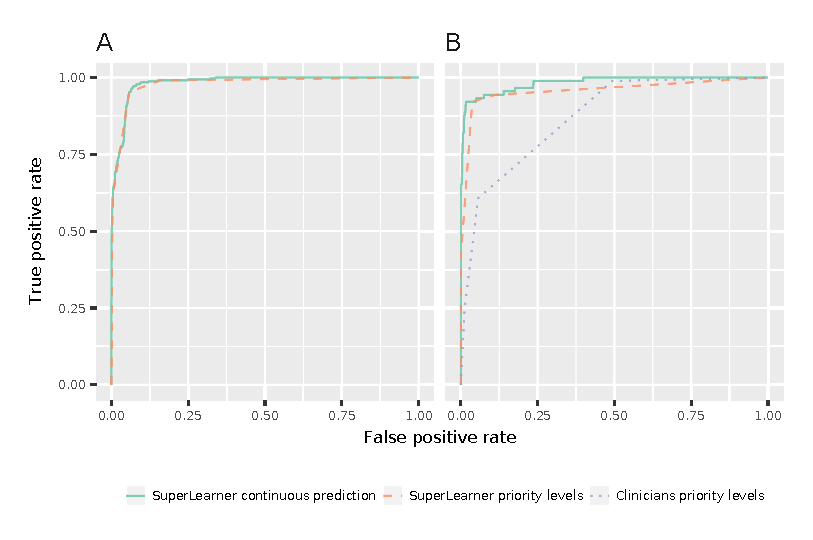
\includegraphics{roc_plot.eps}
  \caption{\bf Receiver operating characteristics curves in training (A) and test
    (B) samples}
  \label{fig:roc_plot}
\end{figure}

\begin{figure}[!h]
  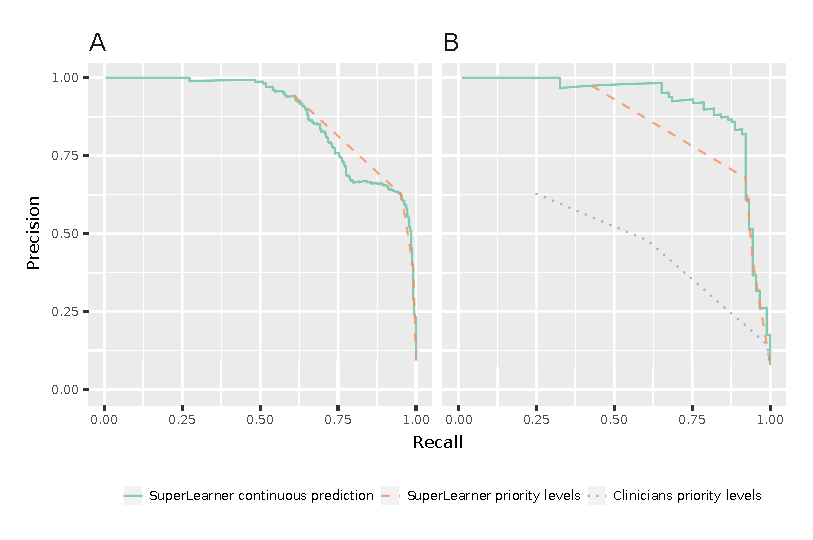
\includegraphics{prec_rec_plot.eps}
  \caption{\bf Precision-recall curves in training (A) and test (B) samples}
  \label{fig:prec_rec_plot}
\end{figure}

We then applied the SuperLearner to the test sample. The AUROCC of the
continuous SuperLearner prediction was 0.9828 (Fig
\ref{fig:roc_plot}B). The performance of each included learner is available as
supporting information in \nameref{S3_Fig} and \nameref{S4_Table}. We used the
same cutpoints as in the training sample to bin the continuous predictions into
the four priority levels. The AUROCC of the SuperLearner priority levels in the
test sample was 0.9574. Fig
\ref{fig:prec_rec_plot}B shows the precision-recall curves in the test sample.

In the test sample we compared the performance of the binned SuperLearner
prediction with that of clinicians. The AUROCC of priority levels assigned by
clinicians was 0.8727. The difference in AUROCC between the
SuperLearner priority levels and clinicians was
-0.0846 (95\% CI -0.1228 - -0.0451). The net reclassification in events and
non-events were 0.0114 (95\% CI -0.0185 - 0.0299) and 0.3500 (95\% CI 0.2405 - 0.6895) respectively. The overall
reclassification is shown in Table \ref{tab:reclass_all}.

% latex table generated in R 3.3.3 by xtable 1.8-2 package
% Fri Jun  1 13:16:50 2018
\begin{table}[!ht]
\centering
\caption{\bf Priority levels assigned by SuperLearner and clinicians in complete test sample (n = 1137)} 
\label{tab:reclass_all}
\begin{tabular}{llllllll}
  \hline
  & \multicolumn{4}{c}{SuperLearner} \\
 Clinicians & Green & Yellow & Orange & Red & Rec. \% & Rec. up \% & Rec. down \% \\
 \hline
Green & 522 & 7 & 3 & 0 & 2 & 2 &  \\ 
  Yellow & 369 & 68 & 46 & 9 & 86 & 11 & 75 \\ 
  Orange & 30 & 7 & 31 & 10 & 60 & 13 & 47 \\ 
  Red & 13 & 0 & 2 & 20 & 43 &  & 43 \\ 
   \hline
\end{tabular}
\caption*{Reclassification (Rec.) figures refer to \% of patients reclassified by the SuperLearner compared to clinicians. Rec. up and Rec. down indicates \% of patients reclassified to a higher or lower priority level respectively.} 
\end{table}


Fig \ref{fig:mortality_plot} shows that the number of patients assigned to each
priority level differed substantially between the SuperLearner and
clinicians. This difference was particularly marked in the green and yellow
priority levels. The SuperLearner assigned the green priority level to
934 patients whereas clinicians assigned this
level to 532 patients. Among the patients that
the SuperLearner prioritised as green 5
died. The corresponding figure for the clinicians was
1. In contrast, the SuperLearner assigned the
yellow priority level to 82 patients, out of
which 2 died. Corresponding figures for the
clinicians were 492 and
34.

% **** Mortality plot
\begin{figure}[!h]
  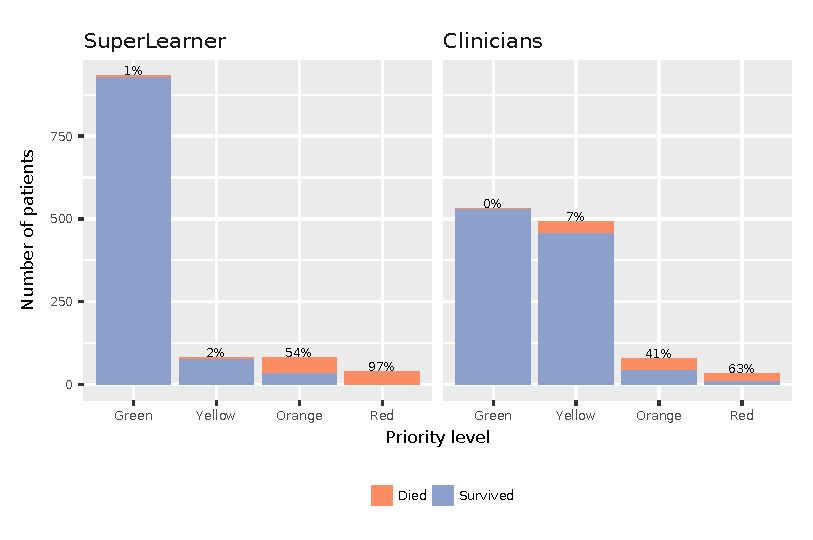
\includegraphics{mortality_plot.eps}
  \caption{\bf Number of patients assigned to each priority level by the SuperLearner and clinicians in the test sample. Percentages are \% with all cause 30-day mortality at each level.}
  \label{fig:mortality_plot} 
\end{figure}


% % Place tables after the first paragraph in which they are cited.
% \begin{table}[!ht]
% \begin{adjustwidth}{-2.25in}{0in} % Comment out/remove adjustwidth environment if table fits in text column.
% \centering
% \caption{
% {\bf Table caption Nulla mi mi, venenatis sed ipsum varius, volutpat euismod diam.}}
% \begin{tabular}{|l+l|l|l|l|l|l|l|}
% \hline
% \multicolumn{4}{|l|}{\bf Heading1} & \multicolumn{4}{|l|}{\bf Heading2}\\ \thickhline
% $cell1 row1$ & cell2 row 1 & cell3 row 1 & cell4 row 1 & cell5 row 1 & cell6 row 1 & cell7 row 1 & cell8 row 1\\ \hline
% $cell1 row2$ & cell2 row 2 & cell3 row 2 & cell4 row 2 & cell5 row 2 & cell6 row 2 & cell7 row 2 & cell8 row 2\\ \hline
% $cell1 row3$ & cell2 row 3 & cell3 row 3 & cell4 row 3 & cell5 row 3 & cell6 row 3 & cell7 row 3 & cell8 row 3\\ \hline
% \end{tabular}
% \begin{flushleft} Table notes Phasellus venenatis, tortor nec vestibulum mattis, massa tortor interdum felis, nec pellentesque metus tortor nec nisl. Ut ornare mauris tellus, vel dapibus arcu suscipit sed.
% \end{flushleft}
% \label{table1}
% \end{adjustwidth}
% \end{table}

% ** Discussion
\section*{Discussion}
Our study suggest that in terms of classification an ensemble machine learner
developed with the SuperLearner may be non-inferior to clinicians to prioritise
among adult trauma patients in the ED. Further, the ensemble learner is superior
to clinician gestalt in terms of discrimination. We have not been able to
identify any previous study that has applied machine learning to prioritise
among trauma patients in the ED. Hence, as far as we know this is the first
study of its kind in this area and we hope that our results can work as
benchmarks to which future work can be compared.

We found that the SuperLearner reclassified non-events to a lower priority
level, compared to clinicians, as indicated by the net reclassification in
non-events. Specifically, the SuperLearner reclassified a majority of patients
from the yellow priority to the green priority level. This is analogous to
reduced overtriage. Overtriage and undertriage are concepts used extensively in
the trauma literature. Undertriage refers to for example patients with major
trauma not being transferred to a trauma centre and overtriage to patients with
minor trauma being transferred to a trauma centre. Our findings indicate that
most of the patients assigned to the yellow priority level by clinicians were
overtriaged and strain the health system in face of limited resources. The
SuperLearner may have the potential to reduce this overtriage substantially.

Three studies have used MMTH learners to limit under and overtriage of trauma
patients.  Talbert et al. applied a tree based learner but found no improvement
over standard criteria \cite{Talbert2007}. More recent research by Follin et
al. demonstrated superior performance of the tree based learner compared to a
model based on logistic regression \cite{Follin2016}. Pearl et al. used neural
networks but could not demonstrate a difference \cite{Pearl2008}. Only Follin
report performance measures that can be compared to our results. Their learner
achieved an AUROCC of 0.82, which is substantially lower than that of our
ensemble learner.

In contrast, the literature is replete with studies using MHTM learners to
reduce under and overtriage, or predict trauma mortality \cite{Rehn2011,
  DeMunter2017,VanRein2018}. The performance of these learners vary
substantially, but many studies report AUROCCs that approaches that of our
ensemble learner. For example, Miller et al. and Kunitake et al. achieved
AUROCCs of almost 0.97 and 0.94 with their models based on logistic regression
\cite{Miller2017}. Neither of these studies however approached the problem of
prioritising among trauma patients in the ED, or suggested how the models could
be used to assign patients to different priority levels.

Our study was limited by the relatively small sample size. For example, we did
not have enough data to run centre wise analysis, which should be a focus of
future studies. Instead we concentrated on data quality and had dedicated
project officers record all data. This resulted in very low levels of missing
feature data. We did however have a considerable amount of missing outcome data,
with about 20\% of patients being lost to follow up. We handled this missingness
using list wise deletion, aware of the potential bias introduced by this
approach. One alternative would have been to use multiple imputation to replace
missing values, however we had no way of determining the mechanism underlying
the missing outcomes why results based on multiple imputed data might be biased
as well. Further, we did not consider it computationally feasible to combine
multiple imputation and bootstrapping for uncertainty estimation. We do however
consider it a strength of our study that the outcome included out of hospital
deaths, when comparably recent research does not \cite{Levin2018, Kunitake2018}.

We used point measurements to train the SuperLearner, meaning that we could
not account for potential changes in patients' clinical condition between the
time when feature and outcome data were collected. The clinicians were however
also limited to the data available when they decided on a priority level,
although this could have included laboratory or imaging findings from a
transferring health facility. Future research may improve the predictions by
both the ensemble machine learner and clinicians by including data from multiple
time points.

As opposed to the clinicians the ensemble learner was limited by the features
that we defined. For example, in our setting with no or very limited electronic
record keeping it would have been challenging to incorporate for example imaging
data. In settings with more extensive electronic records this should be more
feasible. Further, the ensemble learner was limited by the techniques included
in its library. We included a mix of MHTM and MMTH learners, for example
logistic regression and random forest. The performance of our ensemble learner
was already very good, but extending the list of features and techniques
available to the learner would likely improve it further.  Also, we used the
default hyperparameter settings for each technique. Future research may improve
the learner's performance by modifying the included learners' hyperparameters.

Several steps remain before a system to prioritise among adult trauma patients in
the ED based on the SuperLearner can and should be implemented. These steps
involve refining the algorithm, comparing it with other commonly used methods to
prioritise patients in the ED, incorporating it into usable software that may be
used in parallel even in settings with no electronic health records, and
designing an implementation study to assess both its effectiveness and
safety.

There are many ways in which the algorithm could be refined. We regard
optimising the algorithm to minimize deaths in the green priority level as the
most important. Secondly, a sequence in which to measure the variables should be
defined. We think that this sequence should be based on a combination of
individual variable importance and how feasible the variables are to record. We
assume that once this sequence is defined the patients with the most severe
trauma could be identified very quickly using only a small subset of the
variables. Finally, other outcomes should be explored. In a larger dataset a
composite outcome of early deaths, e.g. within 24 hours, and admission to
intensive care or acute surgery could be explored.

\section*{Conclusion}
In terms of classification and discrimination an ensemble machine learning
algorithm developed using the SuperLearner was non-inferior in prioritising
among adult trauma patients in the ED compared to clinician gestalt based on
patients’ presentation. It is possible that the SuperLearner is especially
useful to reduce the number of patients that would be prioritised to a
unnecessarily high priority level.

\section*{Supporting Information}

% Include only the SI item label in the paragraph heading. Use the
% \nameref{label} command to cite SI items in the text.
\paragraph*{S1 Text.}
\label{S1_Text}
{\bf Details of de-identification procedures.}

\paragraph*{S2 Text.}
\label{S2_Text}
{\bf Short descriptions of included learners.}

\paragraph*{S3 Fig.}
\label{S3_Fig}
{\bf Receiver operating characteristic and precision recall curves of included learners.}

\paragraph*{S4 Table.}
\label{S4_Table}
{\bf Risk, weight and area under receiver operating characteristic curve of included learners.}

% \paragraph*{S1 Appendix.}
% \label{S1_Appendix}
% {\bf Lorem Ipsum.} Maecenas convallis mauris sit amet sem ultrices gravida. Etiam eget sapien nibh. Sed ac ipsum eget enim egestas ullamcorper nec euismod ligula. Curabitur fringilla pulvinar lectus consectetur pellentesque.

% \paragraph*{S1 Table.}
% \label{S1_Table}
% {\bf Lorem Ipsum.} Maecenas convallis mauris sit amet sem ultrices gravida. Etiam eget sapien nibh. Sed ac ipsum eget enim egestas ullamcorper nec euismod ligula. Curabitur fringilla pulvinar lectus consectetur pellentesque.

\section*{Acknowledgments}
We would like to thank the Towards Improved Trauma Care Outcomes and the Trauma
Triage Study in India teams.

\nolinenumbers

% Either type in your references using
% \begin{thebibliography}{}
% \bibitem{}
% Text
% \end{thebibliography}
%
% or
%
% Compile your BiBTeX database using our plos2015.bst
% style file and paste the contents of your .bbl file
% here.
% 
\bibliography{bibliography}

\end{document}


%%% Local Variables:
%%% mode: latex
%%% TeX-master: t
%%% End:
